\chapter{Implementation}
\label{chap:implementation}
%This has the description of how you actually went about implementing the project.  This should be focused on the interesting challenges and how those related to the project.

\section{Front-end web development}
\subsection{Overall design implementation}
\label{subsection:frontendOverallDesignImplementation}
%Explain the module pattern
\begin{figure}[h]
\noindent\rule{\textwidth}{1pt}
\begin{lstlisting}[language=JavaScript, caption={Use of Module pattern in stripped down FDG}, label={lst:module}]
var FDG = (function FDG(
    ...
    ) {
        ...
        var getNodeIndex = function(name) { ... }
        ...
        var getNodes = function() { ... }
        ...
        // Expose private functions for global use.
        return {
            getNodeIndex: getNodeIndex,
            getNodes: getNodes,
            ...
        }
    }
);
\end{lstlisting}
\noindent\rule{\textwidth}{1pt}
\end{figure}


% Team background oop.
The team have background in \gls{oop} and very limited experience with JavaScript. Implementation of \gls{frontend} started off as simple functionalities but become a problem as the team progressed. \Gls{frontend} was responsible of many thing such as \gls{fdg}, graphics, \gls{gui} and etc. It became a problem that code was expanding and the team did not know how to control files size but also how to properly divide the code sections in different files.
During refactoring team had done research and found different design pattern where module pattern \cite{scotch:javascriptpatterns} was very similar to classes encapsulation and felt a natural and easy choice to encapsulate functionalities in modern JavaScript fashion. One reason to choose module pattern was that the team wanted \gls{frontend} to be object-oriented, so that only the object would know about its properties and functionalities. Another reason to do so, is that it makes code easliy understandable by use of getters and setters functionalities, as shown in the figure \ref{lst:module}.
The team decided to implement module pattern to structure front-end code. 

There were two libraries used in \gls{frontend}, such as THREE.js and Imgui-js. Three.js is recommended \cite{cmarix:threejs} 3D graphics library as is based on WebGL. It also contains many different functionalities such as scenes, meshes, camera, lights and many more. This fits our requirements and worked for our purpose. Dear ImGUI is a windowing library for C++ that all team members are known of from graphics programming course \cite{course:graphics}. Dear ImGUI has a binding to JavaScript called ImGUI-js that uses TypeScript and Emscripten. This way we were able to integrate ImGUI-js into the system. The library is easy to use and fits our purpose.

\subsection{Force-directed graph}
The \gls{fdg} object maintains a tree of nodes and manage the inter-dependencies between nodes in the tree. It references the tree through its root, which in turn reference its children. The main force calculation and scope handling is done in nodes, so the \gls{fdg} functions as a wrapper.

\subsubsection{Position calculation}

\newglossaryentry{hookesLaw}{name={Hooke's law}, description={Describes a relationship between spring comression and force applied \cite{hooke1678}}}
\newglossaryentry{logit}{name={logit}, description={Inverse of the Sigmund function \cite{wordpress:logitandsigmoid}}}
\newglossaryentry{sigmoid}{name={sigmoid}, description={This is used to transform values on $(-\infty, \infty)$ into numbers on $(0, 1)$ \cite{wordpress:logitandsigmoid}}}

%Explain Logit and force. Could probably add graph from ProfProg rapport.
\begin{figure}[H]
\noindent\rule{\textwidth}{1pt}
\begin{lstlisting}[language=JavaScript, caption={Force calculation FDG}, label={lst:getTotalForce}]
    ...
    if (typeof link !== "undefined") { // Attractive forces
        forceScalar = (
            link.attraction * Math.log10(
                dist / (minDistance + size + node.getSize())
            )
        );
    } else {    // Repulsive force.
        forceScalar = (-1 *
            (
                (maxDistance + size + node.getSize()) /
                Math.pow(dist, 2)
            )
        );

    }
    ...
gravityForce = (Math.log10(distanceFromOrigin + maxSize) - Math.log10(maxSize - distanceFromOrigin)) * gravityForce;
...
\end{lstlisting}
\noindent\rule{\textwidth}{1pt}
\end{figure}

%// Attractive forces are based on logarithmic spring strenghts.
%// Repulsive forces are based on Hookes law (inverse square law).
To calculate the position, \gls{fdg} consider the root as the projects global scope, extracts its children and calculate the force between them. Each child is itself a scope within its parent. The force within each scope is calculated separately to assure that the structure stays within its scope. Listing \ref{lst:getTotalForce} shows that the force calculation depend on whether or not there is a link between the nodes. If there is a link, it is considered a positive attraction, otherwise it is considered a repulsion. 

The idea behind the attractive force calculation is a spring; more energy is required the further apart they are. \gls{hookesLaw} was considered for the calculation. The implemented calculation uses log on distance between each node divided by the minimum distance and size of each data-structure to create a repulsion when the two structures are too close and a strong attraction when they are far apart. 

The repulsion uses the inverse square law to grow weaker over a distance.

\begin{figure}
    \centering
    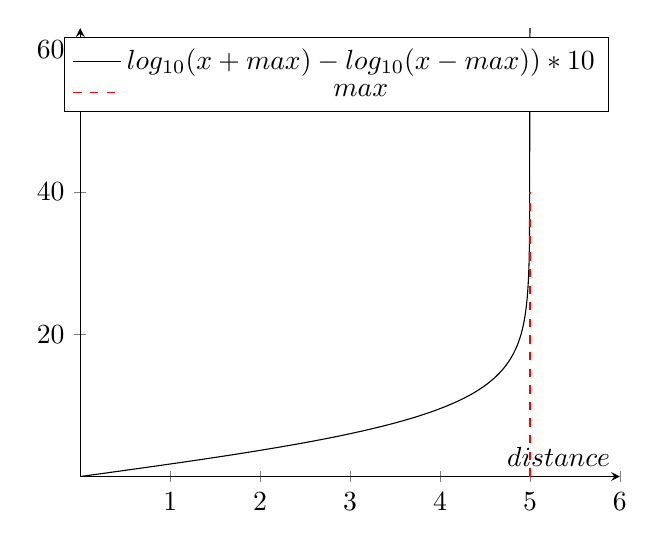
\begin{tikzpicture}
     \begin{axis}[ 
        xlabel={$distance$},
        ylabel={$force$},
        axis lines=middle,
        xmin=0,
        xmax=6,
      ] 
        \addplot[samples=1000, domain=0:5] {(log10(x + 5) - log10(5 - x))*10}; 
        \addlegendentry{$log_{10}(x + max) - log_{10}(x - max)) * 10$}
        
        \addplot +[mark=none, dashed] coordinates {(5, 0) (5, 40)};
        \addlegendentry{$max$}
      \end{axis}
    \end{tikzpicture}

    \caption{Gravity equation based on logit.}
    \label{fig:gravityPlot}
\end{figure}
The figure also show the gravity force calculation. Gravity attracts all structures towards the center of their scope. The center is the zero vector and updated with parents position when added to the scene graph after all relative positions have been calculated. The gravity calculation is based on \gls{logit}, as this implementation gives a gravity force approaching infinity when distance between structures approach max distance. This infinite force prevents structures from escaping their parent scope. The group choose to base it on \gls{logit} as the problem of limiting the position within a scope seemed related to \gls{sigmoid} that the group had experience with through REA1121 - Mathematics for Programming \cite{course:progMath}. \Gls{sigmoid} seemed relevant as it allowed for manipulation of the range and gave a smooth curve. Problem with \gls{sigmoid} is that if $x$ is distance and $y$ is force, then it would clamp on force rather than distance. \gls{logit} was described as the inverse of \gls{sigmoid} and would therefore clamp on distance, limiting the structure within its scope. As the distance between center and a structure could not be zero and gravity should never be negative, \gls{logit} was altered so it crossed the x axis at origin and approached infinity when it approached max distance like shown in figur \ref{fig:gravityPlot}.

\subsubsection{Recursivity of node}
\label{subsubsec:recuriviryOfNode}
%Explain the use of local/global index.
\tikzset{
    vertex/.style = {
        circle,
        fill            = black,
        outer sep = 2pt,
        inner sep = 1pt,
    }
}
\begin{figure}[H]
    \centering
    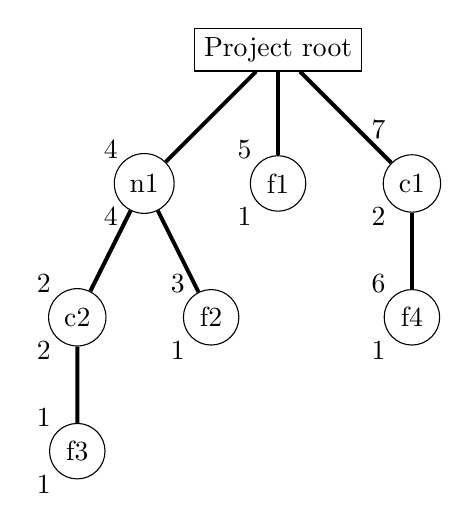
\begin{tikzpicture}[scale=0.85]
        % root
        %\node at (0.0, 1.0) {Project root};
        \node[draw] (root) at (0.0, 0.0) {Project root};
        
        %root scope
        %\node at (4, 1.0) {level 1}; 
        \node[draw, circle] (n1) at (-2, -2) {n1};       \draw[line width=0.5mm,draw=black] (root) to (n1);
        \node at (-2.5, -2.5) {4};    \node at (-2.5, -1.5) {4};
            \node[draw, circle] (c2) at (-3.0, -4.0) {c2};   \draw[line width=0.5mm,draw=black] (n1) to (c2);
            \node at (-3.5, -4.5) {2};    \node at (-3.5, -3.5) {2};
                \node[draw, circle] (f3) at (-3.0, -6.0) {f3};   \draw[line width=0.5mm,draw=black] (c2) to (f3);
                \node at (-3.5, -6.5) {1};    \node at (-3.5, -5.5) {1};
            \node[draw, circle] (f2) at (-1.0, -4.0) {f2};   \draw[line width=0.5mm,draw=black] (n1) to (f2);
            \node at (-1.5, -4.5) {1};    \node at (-1.5, -3.5) {3};
        \node[draw, circle] (f1) at (0, -2.0) {f1};    \draw[line width=0.5mm,draw=black] (root) to (f1);
        \node at (-0.5, -2.5) {1};    \node at (-0.5, -1.5) {5};
        \node[draw, circle] (c1) at (2, -2.0) {c1};     \draw[line width=0.5mm,draw=black] (root) to (c1);
        \node at (1.5, -2.5) {2};    \node at (1.5, -1.2) {7};
            \node[draw, circle] (f4) at (2.0, -4.0) {f4};   \draw[line width=0.5mm,draw=black] (c1) to (f4);
            \node at (1.5, -4.5) {1};    \node at (1.5, -3.5) {6};
        
        
    \end{tikzpicture}
    \caption{local to global index example}
    \label{fig:treeIndex}
    \medskip
    \small
    Figure shows a project with one namespace, one class and one function in global-scope, one class in the namespace and one function in each class. Top number is global-index and lower number is local-index.
\end{figure}
\begin{figure}[H]
\noindent\rule{\textwidth}{1pt}
\begin{lstlisting}[language=JavaScript, caption={Recursive to get node in tree, initiated by FDG(root)}, label={lst:getNode}]
    /**
     * Gets the node based on index.
     *
     * @param  {number} requestedIndex - The requested node index
     * @return {object} The node.
     */
    var getNode = function(requestedIndex, level){
        var localOffset = 0;                // Used to calculate relative index.
        var requestedNode = null;
        // Check if self is requested node.
        if (typeof index !== "undefined" && (index-1 === requestedIndex)) { 
            return this
        }
        // Check if children is requested node.
        children.every( function(child, i) { 
            localIndex = child.getIndex();
            // Check if requested is within childs range.
            if ((localIndex-1)+localOffset < requestedIndex){               
                localOffset += localIndex;
            }else {
                // Child cointain range with requested node.
                requestedNode = child.getNode(requestedIndex - localOffset);
                return false;
            }
            return true;
        });
        return requestedNode;       // indicate that node was not found
    }
\end{lstlisting}
\noindent\rule{\textwidth}{1pt}
\end{figure}
The \gls{fdg} tree requiers each node to have an identifier so that thy can identify each other for linking and potentially other purposes. This identifier is based on position in the tree and for easy searching. The identifier acts as an index in an array, starting at 0 and increasing with one for each node. When it was implemented, it had to be created based only on information of its sub-tree. This means its global index in the tree could not be calculated, only its local index where the node is the root. Once the tree is set in the \gls{fdg}, all nodes are given their global index. Before the global index is given, it can be calculated from the root node by using the local index given while building the tree. The local index is one greater than the sum of each child's local index. Figure \ref{fig:treeIndex} shows the relationship between local and global index while listing \ref{lst:getNode} shows a recurcive call to find a node with global index using the local index. LocalOffset in listing \ref{lst:getNode} refers to the offset from global index and local index caused by the parent node having a subtree to the left of the node being checked. Figure \ref{fig:treeIndex} is simplified by counting from  one instead of zero. The actual global index starts at zero to fit with array index. To account for the local index going from one and global index being accessed from zero, figure \ref{lst:getNode} shows index and local-index being subtracted by one in the conditionals.

\subsection{Localization}
\newglossaryentry{localization}{name={localization}, description={Translating a product into different languages or adapting a product to a country or region}}

\begin{figure}[H]
\noindent\rule{\textwidth}{1pt}
\begin{lstlisting}[language=JavaScript, caption={Language option functionality}, label={lst:locale}]
var LOCALE = (function() {
    var locale = {
        sentences: [
            {
                id: "language_not_found",
                values: [
                    {
                        language: "english",
                        value: "Could not find language"
                    },
                    {
                        language: "norwegian",
                        value: "Fant ikke spr\aket"
                    }
                ]
            },
            ...
        ]
    };

    // Available languages.
    const languages = ["english", "norwegian"];
    
    // English language as defualt.
    var currentLanguage = languages[0];
    
    var getSentence = function(id) { ... }
    ...
})();
\end{lstlisting}
\noindent\rule{\textwidth}{1pt}
\end{figure}

A common feature professional software includes to reach and benefit as many people as possible is \gls{localization} \cite{souphavanh2005localization}. To achieve this, a small system was implemented, where contributors could add sentences in specific languages to a \gls{json} structure, select a language in code and retrieve the added sentences. Even though the functionality for selecting the language exists, the \gls{ui} for selecting the language and updating the \gls{gui} in the visualization it self doesn't exists. The reason for this is that the \gls{gui} got a lower priority than the parsing and visualization. 

The current implementation of \gls{localization} is not very good due to the way sentences are stored. Sentences are stored as objects within a list, where each sentence has a list of the different languages and the sentence it self in that language. To find a sentence, one first have to find the correct sentence based on the identifier and then find the correct language based on the currently selected language. As more sentences are localized, the time taken to find the latter sentences is greatly increased due to the number of sentences to search through. A better way of implementing this would be to sort primarily on the languages them selves in a \gls{keyvaluemap}, where key is the language and value is a list of sentences. This would eliminate the use of list for languages and making the search process more effective. To optimize even further, the sentence list inside the \gls{keyvaluemap} could also be made into a \gls{keyvaluemap}. 

"getSentence" is the function responsible for fetching sentences in the currently selected language. If the sentence could not be found it defaults to the English language. 

\subsection{Graphics}
\label{subsection:graphicsFunctionLinking}
\newglossaryentry{scenegraph}{name={scene graph}, description={A collection of nodes in a graph or tree structure which arranges the logical and often spatial representation of a graphical scene \cite{dollner2000generalizedSceneGraph}}}

\begin{figure}[H]
\noindent\rule{\textwidth}{1pt}
\begin{lstlisting}[language=JavaScript, caption= {Linking function for calls}, label={lst:callLinks}]
var setLinks = function(tree, scene){
    scene.updateMatrixWorld();
    var nodes = tree.getSuccessors();

    nodes.forEach( function(node, index) {

        if (node.getDrawableIndex() != -1) {

            node.getLinks().forEach( function(strength, otherIndex) {

                if (nodes[otherIndex].getDrawableIndex() != -1) {

                    var material = new THREE.LineBasicMaterial({
                        color: STYLE.getDrawables().link.color
                    });

                    var geometry = new THREE.Geometry();

                    geometry.vertices.push(
                        new THREE.Vector3().setFromMatrixPosition(drawables.get(node.getType())[node.getDrawableIndex()].getMesh().matrixWorld),
                        new THREE.Vector3().setFromMatrixPosition(drawables.get(nodes[otherIndex].getType())[nodes[otherIndex].getDrawableIndex()].getMesh().matrixWorld)
                    );

                    var line = new THREE.Line(geometry, material);
                    scene.add(line);
                }
            });
        }
    });
}
\end{lstlisting}
\noindent\rule{\textwidth}{1pt}
\end{figure}

% The sequence of the paragraphs has to be looked at

% Introduce THREE.js?

% Scene graph
\href{https://threejs.org/}{THREE.js} uses a scene structure called \gls{scenegraph}. The structure in the \gls{scenegraph} allows to put object in a hierarchy and if the parent moves in the world, the children follow, to retain their position in relation to their parent. 

% Difficulties in linking
The \gls{scenegraph} caused a lot of confusion in linking the different functions based on calls. The solution for this was to use the \href{https://threejs.org/docs/#api/en/core/Object3D.updateMatrixWorld}{updateMatrixWorld} function from \href{https://threejs.org/}{THREE.js}'s \href{https://threejs.org/docs/#api/en/core/Object3D}{Object3D} which is the base class of \href{https://threejs.org/docs/#api/en/scenes/Scene}{Scene}. It runs a full update on all objects within the \gls{scenegraph} and updates all world positions. After this, it's possible to use \href{https://threejs.org/docs/#api/en/math/Vector3.setFromMatrixPosition}{setFromMatrixPosition} function from \href{https://threejs.org/}{THREE.js}, which uses the world matrix to calculate the actual position from world origin. 

Drawing of objects in \href{https://threejs.org/}{THREE.js} can be done by using the \href{https://threejs.org/docs/#api/en/objects/Mesh}{Mesh} object. This object takes a \href{https://threejs.org/docs/#api/en/core/Geometry}{Geometry} which is the shape made from vertices, and a \href{https://threejs.org/docs/#api/en/materials/Material}{Material} which gives the object characteristics and functionalities, e.g. Phong shading \cite{acm:phongShading1986article}, shadow mapping \cite{acm:perspectiveShadowMap2002article} capabilities, opacity, etc. These can then be added to the scene and updated if needed. 

The generation of the links is performed by looping over each nodes links and fetching the respective node's world position. These positions are given to a \href{https://threejs.org/}{THREE.js} \href{https://threejs.org/docs/#api/en/core/Geometry}{Geometry} and combined with a \href{https://threejs.org/docs/#api/en/materials/LineBasicMaterial}{LineBasicMaterial} object. This results in a line between the two positions. % Last sentence is probably unecessary

% Shapes
Within the visualization there are a bunch of shapes. Each shape represents some kind of data-structure, e.g. class, function, etc. Instead of building custom shapes, it was decided to use \href{https://threejs.org/}{THREE.js} built-in geometries. 

% Mention use of STYLE for color-scheme
The style feature is implemented in the same way as the localization. It contains a \gls{json} data-structure which has a list of color schemes and shape settings. The JavaScript Module pattern was used so the configuration data-structure could be encapsulated to maintain a god structure and keep the application as object oriented as possible. 

% More of a discussion section?
The group wanted the appearance of the application to be customizable to the different vendors, if they have a certain color scheme or style they follow or high contrast styles which highlights different aspects of the program better for those with visual disabilities. Colorblindness could be mitigated by using different shapes for the separate data-structures and a high contrast as well as colorblindness-specific color schemes. These color schemes are not currently implemented, but they will be if any work is continued. The only color schemes added are a SublimeText-inspired scheme and a CodebaseVisualizer3D-based scheme.

% Camera and lighting

\subsection{Interaction}
\newglossaryentry{raycast}{name={raycast}, description={The use of ray–surface intersection tests to solve a variety of problems in computer graphics and computational geometry. \cite{wiki:raycasting}}}

\begin{figure}[H]
\noindent\rule{\textwidth}{1pt}
\begin{lstlisting}[language=JavaScript, caption={A snippet of raycast onMouseClick}, label={lst:onClick}]
/**
 * On click mouse event function.
 *
 * @param      {Event}  event   The event.
 */
function onMouseClick(event) {

    // calculate mouse position in normalized device coordinates
    // (-1 to +1) for both components
    mouse.x = (event.clientX / window.innerWidth) * 2 - 1;
    mouse.y = - (event.clientY / window.innerHeight) * 2 + 1;

    // update the picking ray with the camera and mouse position
    raycaster.setFromCamera(mouse, camera);

    // calculate objects intersecting the picking ray
    var intersects = raycaster.intersectObjects(scene.children ,true);

    if(intersects !== "undefined" && intersects.length > 0) {
        var funcName = intersects[0].object.name.substr(0, intersects[0].object.name.indexOf(' |'));

        sendGetRequest("http://" + config.serverInfo.api_ip + ":" + config.serverInfo.api_port +
            "/repo/" + id + "/file/read/?lineStart=" + functionModels.get(funcName).getStartLine() +
            "&lineEnd=" + functionModels.get(funcName).getEndLine() +
            "&filePath=" + functionModels.get(funcName).getFileName())
        .then(json => {
            windowMgr.setDataStructureImplementation(json.implementation);
        });
    }
}
\end{lstlisting}
\noindent\rule{\textwidth}{1pt}
\end{figure}
\newglossaryentry{keyvaluemap}{name={key-value map}, description={An data-structure that maps keys to values}}
\newacronym{dom}{DOM}{Document Object Model}
The interaction that exists in the system is interaction with functions representations and windows. Window such as implementation window where data-structure implementation shown in it won't wrap but will be hidden and can be seen by temporarily expending it through clicking and dragging on the lower right corner of the window. Once released the window will reset to its original layout to not permanently hide the visualization.

The interaction with data-structures is done using a technique called raycast. Raycast is built into Three.js which is used for mouse picking objects from a 3d space. The function onMouseClick is added as an event listener to JavaScript built in window, which represents window containing \gls{dom} document. As the listing \ref{lst:onClick} shows, first the mouse position is normalized based on screen coordinates, then the raycaster is attached to camera and normalized mouse coordinates are given so that ray is casted from camera to mouse. Once the user clicks in the scene graph a list of intersected object with ray can be fetched. This list is sorted in the order objects were intersected by the ray. This way index 0 of the list will always be object user wants to interact with. The interacted object gives the name of the object that is assigned to object before its added to the scene. A \gls{keyvaluemap} of function models is created, whilst the project json is being parsed in \gls{frontend}. This \gls{keyvaluemap} contains all metadata about all functions that are visualized. This \gls{keyvaluemap} is used to identify the actual model the user has clicked. Once the actual function model is found, it can be used to fetch models implementation and visualize in the implementation window. 

\section{Back-end}

\subsection{Overall design implementation}
\newacronym{url}{URL}{Uniform Resource Locator}
\begin{figure}[h]
\noindent\rule{\textwidth}{1pt}
\begin{lstlisting}[language=go, caption={Api routes}, label={lst:apiRouting}]
// API routings
util.TypeLogger.Info("%s: Setting up api routes", packageName)
router.HandleFunc("/repo/add", controller.RepoController{}.NewRepoFromURI)
router.HandleFunc("/repo/list", controller.RepoController{}.GetAllRepos)
router.HandleFunc("/repo/{repoId}/initial/", controller.RepoController{}.ParseInitial)
router.HandleFunc("/repo/{repoId}/file/read/", controller.CodeSnippetController{}.GetImplementation)
\end{lstlisting}
\noindent\rule{\textwidth}{1pt}
\end{figure}
The \gls{backend} is divided into two parts as mentioned in Technical Design chapter; Go \gls{api} and Java \gls{antlr} parser.

As the listing \ref{lst:apiRouting} shows, some of the entry points has the repository ID as part of their \gls{url}. This \gls{url} path variable is sent from \gls{frontend} and is used to identify repository from database. The placeholder for repository ID is implemented using Gorilla Mux. The idea behind doing this was that the entry point would show what repository should \gls{api} deal with and what operation should be done on it based on \gls{url}. 

The ".../initial/" is the main request that uses \gls{websocket} and communicates with Java \gls{antlr} parser by giving a project file at a time, and expects a \gls{json} with parsed code in return. Whilst being parsed the \gls{frontend} will recieve a message about metadata of the file being processed through "onMessage" channel of \gls{websocket} for server feedback to user. In Go \gls{api} this \gls{json} is added into the project model. Once all project files are parsed the project model is converted into \gls{json} and will be sent as a response to "onClose" channel of \gls{websocket}. 

Initially the plan was to use \gls{antlr} in Golang for parsing and this would have worked since \gls{antlr} has binding for golang. Whilst the team was trying to integrate \gls{antlr} into golang, it came into focus that grammar files that the team was planning to use had embedded Java code, which would have not worked in Golang. Therefore Java seemed to be natural option to fallback to for parsing and since \gls{antlr} is natively made in Java. The team also had some experience in Java through mobile/wearable programming course \cite{course:mobileWearable} The package "os/exec" in Golang would be used to execute Java \gls{antlr} parser and read its output.

There are two library used in the \gls{backend} such as Gorilla mux and JSONObject.

Gorilla mux is a library that is widely used for \gls{url} routing for Golang projects. This library was mentioned in cloud technology course \cite{course:cloud} in which the team already had understanding of and made it very easy to integrate. 

In Java \gls{antlr} parser JSONObject library was used to construct \gls{json} for each data-structure model. Once every line in code is parsed the file model which contains many different properties such as namespace, will loop over each of
 
% endpoints

% gorilla mux as a librarary
% json in java


\subsection{Processing server in Golang}    \label{subsection:golang}

\subsubsection{REST and WebSocket}
\begin{figure}[H]
\noindent\rule{\textwidth}{1pt}
\begin{lstlisting}[language=Go, caption={Websocket success response}, label={lst:websocketMessageSuccess}]
response := WebsocketResponse{
	StatusText: http.StatusText(http.StatusOK),
	StatusCode: http.StatusOK,
	Body: map[string]interface{}{
		"id":               vars["repoId"],
		"status":           "Parsing",
		"currentFile":      parserResponse.CurrentFile,
		"parsedFileCount":  parserResponse.ParsedFileCount,
		"skippedFileCount": parserResponse.SkippedFileCount,
		"fileCount":        parserResponse.FileCount,
	},
}
\end{lstlisting}
\noindent\rule{\textwidth}{1pt}
\end{figure}
Initially the requirements asked for a \gls{rest} service, but this was loosened in favor of \gls{websocket} to allow for updating the user on progress of lengthy tasks. As \gls{http} responses has more extensive status information than \gls{websocket}, the team decided to use the responses as a wrapper for a trimmed down \gls{http} response with \gls{http}Status code, \gls{http}Status text and body containing the requested information. Listing \ref{lst:websocketMessageSuccess} shows a potential response to update user on status of code-base parsing. It sends \gls{http}Status 200 OK, along with what is being parsed, whether it is parsing, done parsing or has failed parsing, how many files have been found and the ration of files that were parsed or not. Files that are not parsed, might include README.md, \gls{git} files or files with unsupported extensions.  

\subsection{Language parsing in JAVA} \label{subsection:parsingJava}
\begin{figure}[H]
\noindent\rule{\textwidth}{1pt}
\begin{lstlisting}[language=AntlrGrammar, caption={Rule for memberdeclaration}, label={lst:antlrCppGrammarRuleExample}]
memberdeclaration
   : attributespecifierseq? declspecifierseq? memberdeclaratorlist? ';'
   | functiondefinition
   | usingdeclaration
   | static_assertdeclaration
   | templatedeclaration
   | aliasdeclaration
   | emptydeclaration
   ;
\end{lstlisting}
\medskip
\small
Taken from CPP14.g4 \cite{git:cpp14_g4} from the ANTLR grammar \gls{git} repository
\noindent\rule{\textwidth}{1pt}
\end{figure}

Listing \ref{lst:antlrCppGrammarRuleExample} shows the rule defining the syntax for member declaration. 
It specifies that it can be of 7 forms, where each is separated by a vertical bar or OR gate. The first rule specifies that it might contain an attributespeifierseq rule, followed by what might be a declspecifierseq, followed in turn by what might be a memberdeclaratorlist and ends with the ";" character. 

\begin{figure}[H]
\noindent\rule{\textwidth}{1pt}
\begin{lstlisting}[language=Java, caption={If block example}, label={lst:ifBlockExample}]
	protected boolean isVariable(CPP14Parser.SimpledeclarationContext ctx){
		CPP14Parser.InitdeclaratorlistContext initDeclList = null;
		CPP14Parser.DeclaratorContext declarator = null;

		if(ctx.initdeclaratorlist() != null) {
			initDeclList = ctx.initdeclaratorlist();
			if(initDeclList.initdeclarator().declarator() != null) {
				declarator = initDeclList.initdeclarator().declarator();
				if(declarator.ptrdeclarator() != null) {
					if(declarator.ptrdeclarator().noptrdeclarator() != null) {
			            if(declarator.ptrdeclarator().noptrdeclarator().declaratorid() != null) {
							return true;
						}
					}
				}
			}
		}

		return false;
	}
\end{lstlisting}
\noindent\rule{\textwidth}{1pt}
\end{figure}
As the grammar file defines the structure of the program, it was highly desired that as much of the parsing as possible be handled by \gls{antlr}. If \gls{antlr} handled the scoping and definitions then one could be very certain that no data-structure was skipped or mishandled. Listing \ref{lst:ifBlockExample} shows an example of where checking for variables is done manually, rather then relying on more listeners in given by \gls{antlr}. This can create a lot of nested if statements to check what form of the rule or nested rule is being matched. This increase the \Gls{cyclomaticcomplexity} and probability of error while also relying on the development team knowing all the niche aspects of a particular data-structure structure. The same is true when merging the output of rules by defining an interval by using the the start point of a rule and the endpoint of an other. If there are optional rules within the context, then the output can vary greatly. 

% More talk about rules?

\begin{figure}[H]
\noindent\rule{\textwidth}{1pt}
\begin{lstlisting}[language=Java, caption={Antlr CPP listener example}, label={lst:antlrCPPListenerExample}]
public void enterFunctiondefinition(CPP14Parser.FunctiondefinitionContext ctx) {
	...

	FunctionModel functionModel = new FunctionModel(input.getText(interval));
	functionModel.setLineStart(ctx.functionbody().start.getLine());
	functionModel.setLineEnd(ctx.functionbody().stop.getLine());
	this.enterScope(functionModel);
}

public void exitFunctiondefinition(CPP14Parser.FunctiondefinitionContext ctx) {
	Model model = this.exitScope();

	if (model instanceof FunctionModel) {
		this.scopeStack.peek().addDataInModel((FunctionModel) model);
	} else {
		this.enterScope(model);
		... // Print wrong parent model
	}
}
\end{lstlisting}
\noindent\rule{\textwidth}{1pt}
\end{figure}
\begin{figure}[H]
\noindent\rule{\textwidth}{1pt}
\begin{lstlisting}[language=Java, caption={Antlr Java listener example}, label={lst:antlrJavaListenerExample}]
public void enterMethodDeclaration(Java9Parser.MethodDeclarationContext ctx) {
	...// Get interval were function identifier is written.
	
	FunctionModel functionModel = new FunctionModel(input.getText(interval),
			ctx.methodHeader().methodDeclarator().identifier().getText());
    functionModel.setLineStart(ctx.methodBody().start.getLine());
	functionModel.setLineEnd(ctx.methodBody().stop.getLine());
	this.enterScope(functionModel);
}

public void exitMethodDeclaration(Java9Parser.MethodDeclarationContext ctx) {
	Model model = this.exitScope();

	if (model instanceof FunctionModel) {
		this.scopeStack.peek().addDataInModel((FunctionModel) model);
	} else {
		this.enterScope(model);
		... // Print wrong parent model
	}
}
\end{lstlisting}
\noindent\rule{\textwidth}{1pt}
\end{figure}

Listing \ref{lst:antlrCPPListenerExample} and \ref{lst:antlrJavaListenerExample} shows a trimmed down version of the parsing of function definition in C++ and Java respectively. Parsing of the two languages can differ significantly as the naming convention used in the different \gls{antlr} grammar files differ and C++ also has a more flexible syntax. Java grammar might also use different methods for defining lists than C++. 
Due to the differences in Java and C++, they are handled separately based on the file extension. 

Java is read by the JavaParserFacade and interpreted by JavaExtendedListener, while C++ is handled by CppParserFace and CppExtendedListener class. Each of the extended listeners extend from their respective \gls{antlr} listener and are meant to contain common functionality for all types of parsers for their language. Currently only the initial parsers exist. The initial parsers create the initial data used for the main project visualization. 

Both \ref{lst:antlrCPPListenerExample} and \ref{lst:antlrJavaListenerExample} listings show the enter function ending with the enterScope(functionModel) call and the exit functions calling exitScope. The enter function is called when the parser reaches the beginning of its respective rule while the exit is called at the end. With the enterScope being called, all following rules being called would have functionModel in memory and know they are matched within the function rule. The check for whether or not the instance of the model is of the expected type in the exit function, were initially undesirable as with a correct and full implementation of the \gls{antlr} file, there would be no possibility for an unexpected model.
